\documentclass[conference]{IEEEtran}
\usepackage{amsmath}
\usepackage{amssymb}
\usepackage{array}
\usepackage{booktabs}
\usepackage{color}
\usepackage{float}
\usepackage{graphicx}
\usepackage{ifpdf}
\usepackage[utf8]{inputenc}
\usepackage{keyval}
\usepackage{listings}
\usepackage{moresize}
\usepackage{multirow}
\usepackage[numbers,sort&compress,square]{natbib}
\usepackage{paralist}
\usepackage{rotating}
\usepackage{soul}
% \usepackage[style=base]{subcaption}
\usepackage{srcltx}
\usepackage{url}
\usepackage[dvipsnames]{xcolor}
\usepackage{xspace}
\usepackage{wrapfig}
\usepackage{hyperref}
% \usepackage{caption}
\usepackage{enumitem}

\definecolor{listinggray}{gray}{0.95}
\definecolor{darkgray}{gray}{0.7}
\definecolor{commentgreen}{rgb}{0, 0.4, 0}
\definecolor{darkblue}{rgb}{0, 0, 0.6}
\definecolor{purple}{rgb}{0.6, 0, 0.6}
\definecolor{middleblue}{rgb}{0, 0, 0.75}
\definecolor{darkred}{rgb}{0.4, 0, 0}
\definecolor{brown}{rgb}{0.5, 0.5, 0}
\definecolor{dkgreen}{rgb}{0,0.5,0}
\definecolor{orange}{rgb}{1,.5,0}
\definecolor{dandelion}{cmyk}{0,0.29,0.84,0}

\lstset{ 
  backgroundcolor=\color{white},   % choose the background color; you must add \usepackage{color} or \usepackage{xcolor}; should come as last argument
  basicstyle=\ttfamily\footnotesize,        % the size of the fonts that are used for the code
  breakatwhitespace=false,         % sets if automatic breaks should only happen at whitespace
  breaklines=true,                 % sets automatic line breaking
  captionpos=b,                    % sets the caption-position to bottom
  commentstyle=\color{purple},    % comment style
  deletekeywords={...},            % if you want to delete keywords from the given language
  escapeinside={\%*}{*)},          % if you want to add LaTeX within your code
  extendedchars=true,              % lets you use non-ASCII characters; for 8-bits encodings only, does not work with UTF-8
  % frame=single,                    % adds a frame around the code
  keepspaces=true,                 % keeps spaces in text, useful for keeping indentation of code (possibly needs columns=flexible)
  keywordstyle=\color{orange},       % keyword style
  language=python,                 % the language of the code
  morekeywords={*,...},            % if you want to add more keywords to the set
  numbers=left,                    % where to put the line-numbers; possible values are (none, left, right)
  numbersep=5pt,                   % how far the line-numbers are from the code
  numberstyle=\tiny\color{darkgray}, % the style that is used for the line-numbers
  rulecolor=\color{black},         % if not set, the frame-color may be changed on line-breaks within not-black text (e.g. comments (green here))
  showspaces=false,                % show spaces everywhere adding particular underscores; it overrides 'showstringspaces'
  showstringspaces=false,          % underline spaces within strings only
  showtabs=false,                  % show tabs within strings adding particular underscores
  stepnumber=2,                    % the step between two line-numbers. If it's 1, each line will be numbered
  stringstyle=\color{commentgreen},     % string literal style
  tabsize=2,                       % sets default tabsize to 2 spaces
  % title=\lstname                   % show the filename of files included with \lstinputlisting; also try caption instead of title
}

\usepackage[normalem]{ulem}
\makeatletter
\def\cyanuwave{\bgroup \markoverwith{\lower3.5\p@\hbox{\sixly \textcolor{cyan}{\char58}}}\ULon}
\def\reduwave{\bgroup \markoverwith{\lower3.5\p@\hbox{\sixly \textcolor{red}{\char58}}}\ULon}
\def\blueuwave{\bgroup \markoverwith{\lower3.5\p@\hbox{\sixly \textcolor{blue}{\char58}}}\ULon}
\font\sixly=lasy6 % does not re-load if already loaded, so no memory problem.
\makeatother

\usepackage{pgfplots}
\pgfplotsset{compat=newest}
\usepgfplotslibrary{fillbetween}
\usetikzlibrary{patterns}

\usepackage{siunitx}
\DeclareSIUnit{\calorie}{cal}
\usepackage[outline]{contour}

\usepackage{makecell}

%\usepackage{xcolor}

\newif\ifdraft
\drafttrue
\ifdraft
 \newcommand{\N}[1]{\textbf{*** NOTE: #1}\xspace}
 \newcommand{\jhanote}[1]{ {\textcolor{red} { ***SJ: #1 }}}
 \newcommand{\mtnote}[1]{ {\textcolor{orange} { ***MT: #1 }}}
 \newcommand{\note}[1]{ {\textcolor{brown} { *** #1 }}}
 \newcommand{\jdnote}[1]{ {\textcolor{cyan} { ***JD: #1 }}}
 \newcommand{\dwwnote}[1]{ {\textcolor{blue} { ***DWW: #1 }}}
\else
 \newcommand{\N}[1]{}
 \newcommand{\jhanote}[1]{}
 \newcommand{\mtnote}[1]{}
 \newcommand{\jdnote}[1]{}
 \newcommand{\dwwnote}[1]{}
 \newcommand{\note}[1]{}
\fi

\newcommand{\cloud}{cloud\xspace}
\newcommand{\clouds}{clouds\xspace}
\newcommand{\pilot}{Pilot\xspace}
\newcommand{\pilots}{Pilots\xspace}
\newcommand{\pilotjob}{Pilot-Job\xspace}
\newcommand{\pilotjobs}{Pilot-Jobs\xspace}
\newcommand{\pilotcompute}{Pilot-Compute\xspace}
\newcommand{\pilotcomputedescription}{Pilot-Compute Description\xspace}
\newcommand{\pilotdescription}{Pilot-Description\xspace}
\newcommand{\pilotcomputes}{Pilot-Computes\xspace}
\newcommand{\pilotdata}{Pilot-Data\xspace}
\newcommand{\pilotdatadescription}{Pilot-Data Description\xspace}
\newcommand{\pilotdataservice}{Pilot-Data Service\xspace}
\newcommand{\pilotcomputeservice}{Pilot-Compute Service\xspace}
\newcommand{\computedataservice}{Compute-Data Service\xspace}
\newcommand{\computeunitdescription}{Compute-Unit Description\xspace}
\newcommand{\dataunitdescription}{Data-Unit Description\xspace}
\newcommand{\pilotmapreduce}{PilotMapReduce\xspace}
\newcommand{\mrmg}{MR-Manager\xspace}
\newcommand{\pstar}{P*\xspace}
\newcommand{\pd}{PD\xspace}
\newcommand{\pc}{PC\xspace}
\newcommand{\pcs}{PCs\xspace}
\newcommand{\pj}{PJ\xspace}
\newcommand{\pjs}{PJs\xspace}
\newcommand{\pds}{Pilot Data Service\xspace}
\newcommand{\computeunit}{Compute-Unit\xspace}
\newcommand{\computeunits}{Compute-Units\xspace}
\newcommand{\dataunit}{Data-Unit\xspace}
\newcommand{\dataunits}{Data-Units\xspace}
\newcommand{\du}{DU\xspace}
\newcommand{\dus}{DUs\xspace}
\newcommand{\dud}{DUD\xspace}
\newcommand{\cu}{CU\xspace}
\newcommand{\cus}{CUs\xspace}
\newcommand{\cud}{CUD\xspace}
\newcommand{\su}{SU\xspace}
\newcommand{\sus}{SUs\xspace}
\newcommand{\schedulableunit}{Schedulable Unit\xspace}
\newcommand{\schedulableunits}{Schedulable Units\xspace}
\newcommand{\cc}{c\&c\xspace}
\newcommand{\CC}{C\&C\xspace}
\newcommand{\up}{\vspace*{-1em}}
\newcommand{\upp}{\vspace*{-0.5em}}
\newcommand{\numrep}{8 }
\newcommand{\samplenum}{4 }
\newcommand{\tmax}{$T_{max}$ }
\newcommand{\tc}{$T_{C}$ }
\newcommand{\tcnsp}{$T_{C}$}
\newcommand{\bj}{BigJob\xspace}
\newcommand{\irods}{iRODS\xspace}

\newcommand{\I}[1]{\textit{#1}\xspace}
\newcommand{\B}[1]{\textbf{#1}\xspace}
\newcommand{\T}[1]{\texttt{#1}\xspace}
%\newcommand{\C}[1]{\textsc{#1}\xspace}

\newcommand{\mr}[1]{\multirow{2}{*}{#1}}%
\newcommand{\mc}[2]{\multicolumn{#1}{l}{#2}}

\lstdefinestyle{myListing}{
  frame=single,
  backgroundcolor=\color{listinggray},
  %float=t,
  language=C,
  basicstyle=\ttfamily \footnotesize,
  breakautoindent=true,
  breaklines=true
  tabsize=2,
  captionpos=b,
  aboveskip=0em,
  belowskip=-2em,
  %numbers=left,
  %numberstyle=\tiny
}

\lstdefinestyle{myPythonListing}{
  frame=single,
  backgroundcolor=\color{listinggray},
  %float=t,
  language=Python,
  basicstyle=\ttfamily \scriptsize,
  breakautoindent=true,
  breaklines=true
  tabsize=2,
  captionpos=b,
  %numbers=left,
  %numberstyle=\tiny
}



%  \setlength{\parskip}{0.05ex} % 1ex plus 0.5ex minus 0.2ex}
%  \setlength{\parsep}{0pt}
%  %\setlength{\headsep}{0pt}
%  \setlength{\topskip}{0pt}
%  \setlength{\topmargin}{0pt}
%  %\setlength{\topsep}{0pt}
%  \setlength{\partopsep}{0pt}

% This is now the recommended way for checking for PDFLaTeX:


\ifpdf
\DeclareGraphicsExtensions{.pdf, .jpg, .tif}
\else
\DeclareGraphicsExtensions{.ps,  .eps, .jpg}
\fi

\tolerance=1000
\hyphenpenalty=10


\begin{document}


% \title{Alchemical and Endpoint Free Energy Calculations at Scale}

%\title{Rapid, Concurrent and Adaptive Extreme-scale Free energy calculation}

\title{Trading-off Accuracy with Computational Cost: Adaptive Algorithms to Reduce Time to Clinical Insight}



% \author{Jumana Dakka$^{1}$,  Kristof Farkas-Pall$^{3}$, David W. Wright$^{3}$, .... Shantenu Jha$^{1}$$^{,2}$, \\

\author{Jumana Dakka$^{*,1}$, Kristof Farkas-Pall$^{*,2}$, Vivek Balasubramanian$^{1}$ , Matteo Turilli$^{1}$, \\
 Shunzhou Wan$^{2}$, David W Wright$^{2}$, Stefan Zasada$^{2}$, \\\
 Peter V Coveney$^{2}$, Shantenu Jha$^{1,3}$ \\

  \small{\emph{$^{1}$ Rutgers, the State University of New Jersey, Piscataway, NJ 08854, USA}}\\
   \small{\emph{$^{2}$ University College London, London, UK, WC1H 0AJ}}\\
   \small{\emph{$^{3}$ Brookhaven National Laboratory, Upton, New York, 11973}}\\
   \small{\emph{$^{*}$ Contributed Equally}}
}


\date{}
\maketitle

\begin{abstract}

\end{abstract}


% ---------------------------------------------------------------------------
% Introduction
% ---------------------------------------------------------------------------
\section{Introduction}\label{sec:intro}

The efficacy of drug treatments depends on how tightly small molecules bind to their target proteins. Quantifying the strength of these interactions (the so called ‘binding affinity’) is a grand challenge of computational chemistry, the surmounting of which could revolutionize drug design and provide the platform for patient specific medicine. Recently, improvements in computational power and algorithm design mean that reliably quantifying binding affinities from molecular simulation is now becoming a genuine possibility. Exploiting these advances and further refining the technologies involved requires the marshaling of huge simulation campaigns, and impacting clinical or industrial decision making means that computations must be turned around in timescales of hours or days.


% ---------------------------------------------------------------------------
% Scientific Motivation
% ---------------------------------------------------------------------------

\subsection{Scientific Motivation}\label{sec:motivation}

Cancer is the second leading cause of death in the United States, accounting for nearly 25 of all deaths; in 2015, over 1.7 million new cases were diagnosed, with over 580,000 deaths \cite{acs-cancer-facts-2015}. The development of targeted kinase inhibitors—which selectively inhibit kinases involved in signaling pathways that often control growth and proliferation that become dysregulated in many cancers—has changed the way many of these cancers are treated. There are currently 35 FDA-approved small molecule targeted kinase inhibitors in clinical use, and for the past decade, they have represented a significant fraction of the \$37 billion U.S. market for oncology drugs \cite{FDA}. Imatinib, the first of these of drugs, is partially credited for doubling survivorship rates in certain cancers \cite{ACSreport}. Unfortunately, the development of resistance to these drugs limits the amount of time that patients can derive benefits from their treatment. Resistance to therapeutics is responsible for more than 90 of deaths in patients with metastatic cancer \cite{90death}. While drug resistance can emerge via multiple mechanisms, mutations in the therapeutic target drive drug resistance in many patients; in some commonly targeted kinases such as EGFR, missense mutations are the mechanism of resistance in as many as 90 of cases
At the same time, the rapid drop in cost of next-generation sequencing technologies has led many cancer centers to begin deep sequencing patient tumors to identify the genetic alterations driving individual cancers, with the ultimate goal of making individualized therapeutic decisions based upon this data—an approach termed precision cancer therapy. While several common (recurrent) mutations have been cataloged due to their ability to induce resistance or susceptibility to particular kinase inhibitors, the vast majority of clinically observed mutations are rare, essentially ensuring that it will be impossible that catalog-building alone will be sufficient for making therapeutic decisions about the majority of individual patient tumors.

There are two major strategies for countering this threat to treatment efficacy: tailoring the drug regimen received by a patient according to the mutations present in their particular cancer (precision therapy), and development of more advanced second- or third-line therapies that retain potency for known resistance mutations. In both cases, future developments require insight into the molecular changes produced by mutations, as well as ways to predict their impact on drug binding on a timescale much shorter than is typically experimentally feasible.

Molecular simulation based binding affinity calculations represent a practical, quantitative, generalizable approach to predicting the impact of clinically observed mutations on kinase inhibitor affinity. It has been shown that computational methods comparing the binding of different drugs based on molecular dynamics (MD) can now achieve useful predictive accuracy (1 kcal/mol) for well-behaved proteins \cite{shirts-mobley-chodera:2007:annu-rep-comput-chem:prime-time, abel:jacs:2015:fep-plus}. This accuracy is sufficient to greatly accelerate lead optimization \cite{shirts-mobley-brown:2009:sbdd}. Furthermore, recent work also indicates that the same approaches achieve the level of accuracy required to predict the impact of kinase resistance mutations, though published work has only examined single mutations in Abl and FGFR \cite{mondal:jacs:2016:imatinib-gatekeeper,  Bunney2015}.

\subsection{Binding Affinity Calculation Protocols}\label{sec:bac}

Computing accurate protein-drug binding affinities (also known as binding free energies) requires a simulation technique which captures the chemical detail of the system. MD simulations are the time dependent numerical integration of the classical equations of motion for molecular systems. Application of MD to atomistic models of proteins and their ligands can be used to answer questions about the properties of a specific system often more readily than experiments on the actual system. Free-energy calculations in the framework of MD simulations not only yield quantitative estimates of binding strength but also provide insights into the most important interactions driving the process.

Most methods for calculating binding affinities fit into one of two broad classes; so called alchemical and endpoint methodologies. Alchemical free energy calculations employ unphysical (“alchemical”) intermediates to calculate changes in free energies between two systems. It is common in these methods to refer to a variable, $\lambda$, which describes the path taken to transform one protein sequence (or ligand) into another. Endpoint methods, as the name suggests, consider the difference in energy between bound and unbound structures. To obtain information on the differences in binding affinity of different sequences for a panel of kinase inhibitors requires a deployment of various strategies, incorporating both alchemical and endpoint approaches. In this work we deploy approaches from both of these classes.


\subsection{Ensemble Molecular Dynamics}\label{sec:emd}

Statistical mechanics provides the prescription for calculating such macroscopic quantities as ensemble averages of microscopic states. Traditionally, these macroscopic properties have usually been calculated from the time average of a single “long” duration trajectory. An intuitive and potentially more time efficient method to capture the mixing dynamics required to describe an equilibrium thermodynamic state is the use of an ensemble of separate trajectories. \cite{Coveney2016}

The major sources of error in free energy calculations are the representation of the system chemistry encoded in the forcefield used, finite sampling and the free energy estimator. Protocols developed in the Coveney labs have obtained accurate and precise results which successfully reproduce experimental binding free energies from a wide range of systems. \cite{Wright2014, Wan2017brd4, Wan2011, chodera-shirts:jcp:2011:gibbs, Chodera2016} Comparisons of results obtained for a large set of sequences will provide valuable insights on the importance of choices made in simulation and analysis for the overall accuracy and predictive power of free energy calculations, and facilitate the refinement of our protocols.


\subsection{Alchemical Protocol (TIES)}\label{sec:ties}

Alchemical methods employ MD simulations of unphysical, alchemical intermediate states that attenuate the interactions of the small molecule with its environment. These alchemical intermediate states include both the fully-interacting complex as well as replicas in which the ligand does not interact with its environment, and allow the total free energy of binding—including entropic and enthalpic contributions—to be efficiently computed. Typically, the alchemical path between the states of interest is described by a parameter, $\lambda$, which varies between 0 for the initial and 1 for the final state of the transformation of interest. Sampling is then performed at a series of points along this path and the gradient of the energy integrated to calculate the binding affinity.

The TIES (thermodynamic integration with enhanced sampling) protocol, developed within the Coveney lab, employs ensemble sampling at each $\lambda$ window to yield reproducible, accurate, and precise relative binding affinities. \cite{ Wan2017brd4} Based on the direct calculation of ensemble averages, it allows us to determine statistically meaningful results along with complete control of errors. As currently designed, TIES computes the change in binding affinity between two related system (termed ‘relative binding affinities’).


\subsection{Endpoint Protocol (ESMACS)}\label{sec:esmacs}

Computationally cheaper, but less rigorous methods, endpoint methods have been used to directly compute the binding strength of a drug to the target protein sequence from MD simulations (as opposed to differences in affinity). Combining these methods with an ensemble simulation approach has demonstrated the potential to robustly evaluate the impact of mutations on drug binding in both HIV protease \cite{Wright2014} and the EGFR kinase. \cite{Wan2011}

We have developed an ensemble-based endpoint protocol called ESMACS (enhanced sampling of molecular dynamics with approximation of continuum solvent). The protocol is built on the popular molecular mechanics Poisson–Boltzmann surface area (MMPBSA) \cite{MAssova1999} method which makes a continuum approximation for the aqueous solvent in order to obtain results on practical timescales. Commonly, MMPBSA analyses are performed on a single MD trajectory, or even a single structure. We have demonstrated the lack of reproducibility of such an approach in both HIV-1 protease and MHC systems, with calculations for the same protein-ligand combination, with identical initial structure and force field, shown to produce binding affinities varying by up to 12 kcal/mol for small ligands (flexible ligands can vary even more). \cite{Wan2015} ESMACS employs MMPBSA to produce ensemble- based, converged and reproducible, determinations of binding free energies (separate ligand and receptor trajectories can also be used to account for adaptation energies). This provides a rapid quantitative approach sensitive enough to determine changes in binding free energies which differentiate susceptible and resistant sequences (typically of the order of 2 kcal/mol).


\section{Performance Metrics}\label{sec:performance}

TIES is rigorous but computationally expensive and has a limited range of
applicability. ESMACS is approximate but can be employed across any set of
ligands at lower computational cost.

Each of these protocols run a large range of mutations where each
mutation is captured as independent pipelines composed of multiple replicas
where each replica consists of multi-stage short bursts
of simulations, followed by a single replica for analysis. The process is
repeated over a number of iterations depending on the convergence criteria
in the analysis stage. Each replica requires 16 cores, where each pipeline
runs approximately 10 hours, over a range of 100 mutations where each mutations
spawns either 25 or 65 replicas, depending on the protocol.


\section{Computational Challenges}\label{sec:cc}

\jhanote{There is no mention of adaptivity as a challenge. Vivek should add
from his paper.}

\jhanote{Need better organization. Separate out challenge of (i) simple and usable software systems, (ii) scale and interoperability, and (iii) adaptivity challenges. }

High-performance computing (HPC) environments were designed to primarily
support the execution of single simulations. Current HPC platforms enable the
strong and weak scaling of single tasks (hitherto mostly simulations), with
limited software and systems support for the concurrent execution of multiple
heterogeneous tasks as part of a single application (or workflow). As the
nature of scientific inquiry and the applications to support that inquiry
evolve, there is a critical need to support the scalable and concurrent
execution of a large number of heterogeneous tasks.

Sets of tasks with dependencies that determine the order of their execution
are usually referred to as ``workflows''. Often times, the structure of the
task dependencies is simple and adheres to discernible patterns, even though
the individual tasks and their duration are non-trivially distinct. Put
together, it is a challenge to support the scalable execution of workflows on
HPC resources due to the existing software ecosystem and runtime systems
typically found.

Many workflow systems have emerged in response to the aforementioned problem.
Each workflow system has its strengths and unique capability, however each
system typically introduces its problems and challenges. In spite of the many
successes of workflow systems, there is a perceived high barrier-to-entry,
integration overhead and limited flexibility.

Interestingly, many commonly used workflow systems in high-performance and
distributed computing emerged from an era when the software landscape
supporting distributed computing was fragile, missing features and services.
Not surprisingly, initial workflow systems had a monolithic design that
included the end-to-end capabilities needed to execute workflows on
heterogeneous and distributed cyberinfrastructures. Further, these workflow
systems were typically designed by a set of specialists to support large
``big science'' projects such as those carried out at the
LHC~\cite{breskin2009cern} or LIGO~\cite{althouse1992ligo}. The fact that the
same workflow would be used by thousands of scientists over many years
justified, if not amortized, the large overhead of integrating application
workflows with monolithic workflow systems. This influenced the design and
implementation of interfaces and programming models.

However as the nature, number and usage of workflows has evolved so have the
requirements: scale remains important but only when delivered with the
ability to prototype quickly and flexibly. Furthermore, there are also new
performance requirements that arise from the need to support concurrent
execution of heterogeneous tasks. For example, when executing multiple
homogeneous pipelines of heterogeneous tasks, for reasons of efficient
resource utilization there is a need to ensure that the individual pipelines
have similar execution times. The pipeline-to-pipeline fluctuation must be
minimal while also managing the task-to-task runtime fluctuation across
concurrently executing pipelines.

% \mtnote{Should we define what an ensemble is?} \jdnote{We defined ensemble
% in the Methodology Section: We term this approach ensemble molecular
% dynamics, “ensemble” here referring to the set of individual (replica)
% simulations conducted for the same physical system.}

Thus the flexible execution of heterogeneous ensembles MD simulations face
both system software and middleware challenges: existing system software that
is typically designed to support the execution of single large simulations on
the one hand, and workflow systems that are designed to support specific use
cases or `locked-in' end-to-end executions. In the next Section, we discuss
the design and implementation of the RADICAL-Cybertools, a set of software
building blocks that can be easily composed to design, implement and execute
domain specific workflows rapidly and at scale.

\section{Solution}\label{sec:solution}

\jhanote{The Solution is not just HTBAC per se, but the application of HTBAC to the specific problem. The specific problem has not been identified so far. I would propose divided this section into two parts. The first about  HTBAC and its scalability; and the second part about its application to the specific problem.}

The RADICAL Cybertools (RCT), developed by The RADICAL Lab, enables the
efficient and dynamic execution of ensembles on heterogeneous computing
resources. Different from other runtime systems, RCT decouples the workload
execution and resource management details from the expression of the
application, which significantly reduces the burden on the end user.
RCT has been used extensively to support
biomolecular sciences methods and algorithms, e.g., replica exchange, adaptive
sampling and high throughput binding affinity calculations.

Here we describe High Throughput Binding Affinity Calculator (HTBAC),
which builds upon the RADICAl Cybertools, as the framework solution to support
the coordination of the required scale of computations, thereby
allowing us to employ thousands of cores at a time.

Most benchmark evaluations of free energy protocols in the literature look
at only a small number of systems, drawing inferences from tens or hundreds
of runs. HTBAC facilitates studies on unprecedented scales, with the number
of systems investigated an order of magnitude larger than published studies,
which provides the opportunity to gain invaluable knowledge on the domain of
applicability of current MD technologies. In particular, we demonstrate the
use of HTBAC to compute the binding affinities of anti-cancer drugs to their
target proteins (the EGFR kinase) using two simulation protocols with differing
levels of rigor and computational cost, ESMACS and TIES.

HTBAC is not limited to these protocols as additional protocols can be
expressed and implemented easily with the HTBAC user-facing API, however for
demonstration we focus on these ensemble protocols HTBAC has demonstrated
sizable execution and performance of the ESMACS~\cite{dakka2017} and TIES~\cite{dakka_farkaspall} protocols on leadership
class machines including NCSA Blue Waters. For example, we demonstrated how HTBAC
scales almost perfectly to hundreds of concurrent multi-stage pipelines for the TIES 
protocol in ~\ref{fig:weak_scaling}.

\begin{figure}
  \centering
   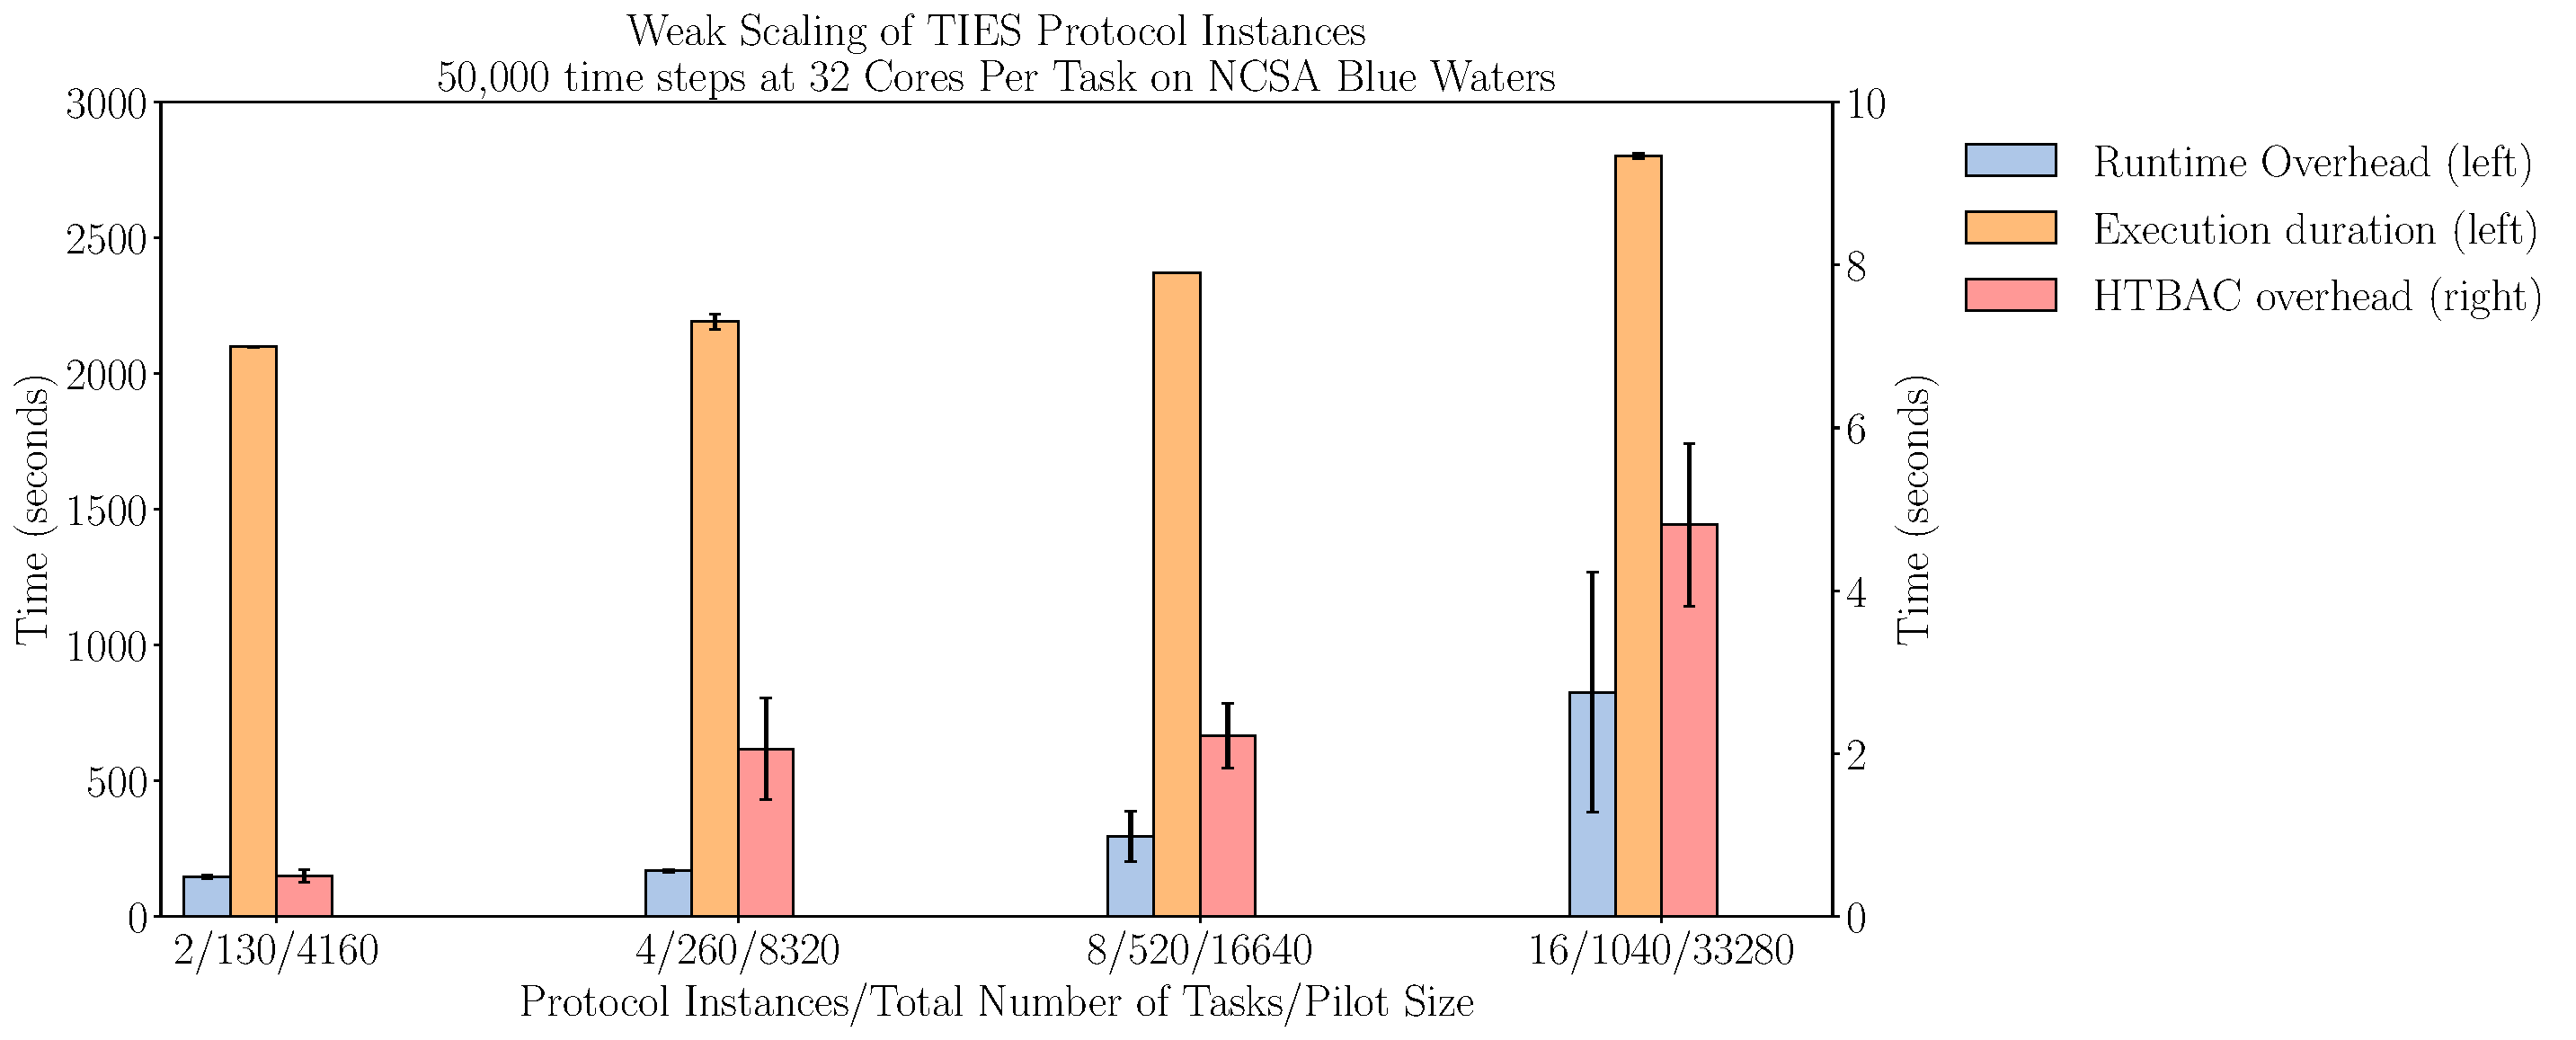
\includegraphics[width=\columnwidth]
   {weak_scaling_TIES_instances_50,000_timesteps_with_16_instances.pdf}
  \caption{Weak scaling properties of HTBAC. We investigate the
  weak scaling of HTBAC as the ratio of the number of protocol instances to
  resources is kept constant. Overheads of HTBAC (right), and runtime overhead 
  (left) and \(TTX\) (left) for experimental configurations investigating the 
  weak scaling of TIES. We ran two trials for each protocol instance 
  configuration. Error bars in \(TTX\) in 2 and 8-protocol runs are 
  insignificant.}
\label{fig:weak_scaling}
\end{figure}

Both ESMACS and TIES have been successfully used to predict binding affinities
quickly and accurately. Nonetheless, they are very expensive computationally,
and optimizing the execution time while still improving the accuracy is
desirable. Given the very large number of drug candidates, it is imperative to
gain maximum insight into potential candidate compounds using time and
resources efficiently. This provides one clear motivation for the use of
adaptive methods which minimize the compute time used whilst producing binding
free energy estimates meeting pre-defined quality criteria (such as
convergence or statistical uncertainty below a given threshold).

This additional driver for \textit{adaptivity} suggest that algorithmic methods will
typically involve compounds with a wide range of chemical properties which can
impact not only the time to convergence, but the type of sampling required to
gain accurate results. In general, there is no way to know before running
calculations exactly which setup of calculation is required for a particular
system. For example in TIES, the number (or the exact location) of the
$\lambda$ windows that will most impact the calculation are not known
\textit{a priori}, and change between physical systems (drugs). As multiple
simulations must be run for each window, sampling with a very high frequency
is expensive and impractical. Furthermore, adaptive placement of $\lambda$
windows is likely to better capture the shape of the
$\partial U/\partial\lambda$ curve, leading to more accurate and precise
results for a given computational cost.

In order to support such
investigations, in addition to being scalable, HTBAC is enhanced to
support flexible resource reallocations schemes where resources can be moved
between simulations run using different protocols or systems, for example,
when one calculation has converged whilst another has not. This adaptability
makes it easier to manage complex programs where efficient use of resources
is required in order to achieve a time to completion of studies comparable to
those of high throughput chemistry.

The novel contributions of HTBAC are: (i) Unprecedented throughput: it allows
the concurrent screening for drug binding affinities of multiple compounds at
unprecedented scales, both in the number of candidates and resources utilized;
(ii) Agile selection of different binding affinity protocols: HTBAC supports
inter-protocol adaptivity, leading to resources being assigned at runtime to
the ``optimal" protocol (as determined by accuracy for given computational
cost); (iii) Support for intra-protocol adaptivity, which provides the
efficient execution of individual protocols.



% While RCT supports concurrent task execution up to 000 tasks on Blue Waters,
% the user is required to translate and codify each of these protocols with the
% corresponding mutation using the EnTK API, and scale these protocols
% based on the desired number of mutations and replicas [9]. We leverage
% the advanced resource management capabilities of RADICAL Cybertools and
% automate this process by providing a native selection of protocols where
% the user only provides the configuration files for each mutation, the number
% of replicas per mutation and the number of cores needed to support each
% protocol. To this effect, the framework uses EnTK to provide a higher level of
% abstraction that allows the user to interface closer to the science problem.


\section{Impact of Solution}\label{sec:impact}


The flexibility provided by HTBAC to run adaptive workflows offers huge advantages scientifically.
Firstly the intra-protocol adaptivity allows the automated optimization of calculations to ensure that
results are obtained with known precision across systems which may exhibit very different behavior (for example levels of `roughness' in the $\partial U/\partial\lambda$ curve in TIES).
This has a significant impact of the reliability of comparisons between runs.
The ability to switch between protocols on the other hand offers a mechanism through which `cheaper' approximate methods (such as ESMACS) can be used to scan large regions of chemical space, whilst more accurate and `expensive' ones are employed to investigate areas of specific interest (TIES).
This maps directly onto processes such as hit to lead optimization in drug discovery and cold be of particular use in investigating activity cliffs.
This is a phenomena where small chemical changes provide large differences in drug efficacy.
If changes are detected using an approximate method it is important to verify that they come from
real chemical effects and not simply inaccuracies in the computational algorithm employed.

The scale enabled by HTBAC also has an impact on the potential for scientific discovery using free energy calculations.
Most studies in the literature are limited to the investigation of tens of protein-ligand complexes.
In order to establish the validity of particular combinations of forcefield and simulation protocol and
quantify uncertainties much larger campaigns are needed.
Our ensemble has already provided evidence that the variability in single runs is sufficient to
swamp true differences between systems of interest.
The combined need for both large numbers of systems and multiple repeats of each one produces a requirement
for middleware to manage huge numbers of simulations.

HTBAC allows the concurrent screening
for drug binding affinities of multiple compounds at unprecedented scales,
both in the number of candidates and resources utilized. Specifically, we
investigated weak scaling behavior for screening sixteen drug candidates
concurrently using thousands of multi-stage pipelines on more than 32,000
cores on NCSA Blue Waters. This permits a rapid time-to-solution that is
essentially invariant with respect to the calculation protocol,
size of target system and number of ensemble simulations. In addition,
HTBAC enabled the adaptive execution of the TIES protocol
providing greater convergence (i.e., lower errors) for a given amount of
computational resources.

These developments fit into a wider vision in which the use of
flexible and responsive computational protocols produce accurate,
precise and reproducible estimates of the free energy of binding with
meaningful error bars. Not only would this allow for wider uptake of
computational techniques in industrial settings but opens up possibilities
of using these technologies in clinical decision support scenarios. By creating
a `digital twin', where the target protein is based on the real patients
genetic sequence, a specific individuals response to different
treatments could be predicted.


\section{Analysis of Solution}\label{sec:analysis}

Our previous work deploying both ESMACS and TIES has typically involved comparing 10 to 20 computed
binding affinities.
An example would be the recent study of BRD4 inhibitors conducted in collaboration by UCL and GSK \cite{Wan2017brd4}, which involved 15 drugs (usually we prepare a similar number of systems using each protocol, here 12 TIES transformations were studied).
Using our non-adaptive protocols each system typically requires approximately 10k and 25k core hours for ESMACS and TIES respectively.
So a 20 compound study (with 20 transforms) would use $\sim$700k core hours.
As previously described this type of study does not meet the size necessary to really impact industrial processes which focus from libraries of potentially millions of compounds down to hundreds of hits which need to be optimized.
HTBAC is designed to enable this types of workflow to be sustained, a development which means that we can now look to conduct the scale of studies necessary to refine protocols and forcefields for production work in drug discovery and refinement.



% ---------------------------------------------------------------------------
% Demonstration
% ---------------------------------------------------------------------------
\section{Demonstration}\label{sec:demo}


% ---------------------------------------------------------------------------
% BIBLIOGRAPHY
% ---------------------------------------------------------------------------
\bibliographystyle{unsrt}
\bibliography{rutgers,ucl,mskcc}

\end{document}
